%Introduction

\begin{figure}[t]
	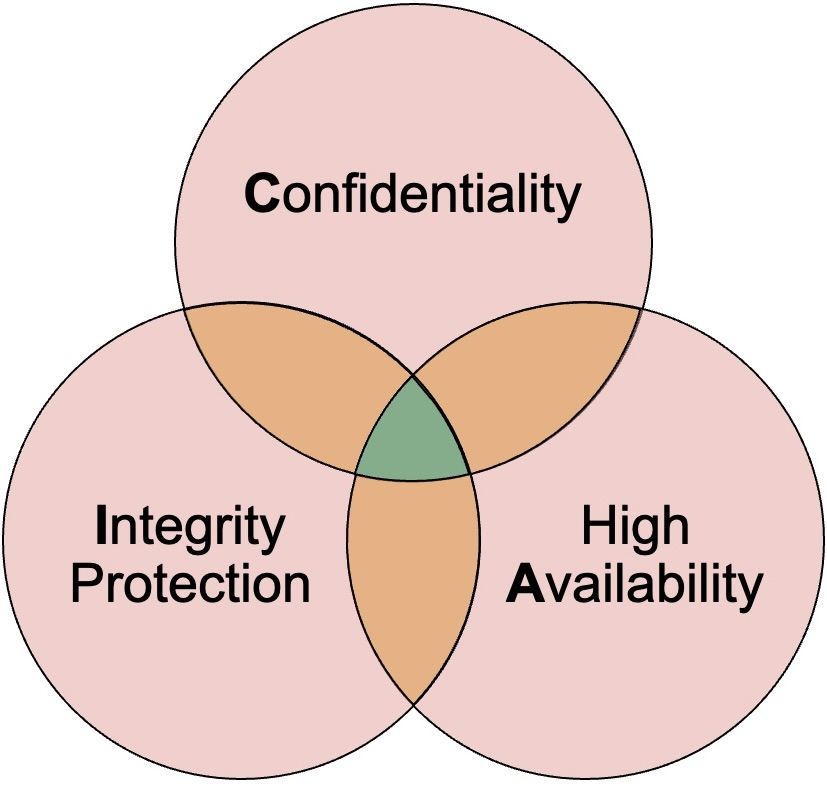
\includegraphics[scale=0.12]{pictures/cia_triad}
	\caption{Graphic of the CIA triad}
	\label{cia}
\end{figure}

\section{Introduction}
Today's applications are increasingly stored in the cloud for more flexibility and scalability. 
 But over the time more and more cloud providers get compromised or data is stolen, because providers did not encrypt this data. This is the reason, finances and health applications that handle sensitive data cannot afford this risk with hosting their applications on the cloud. To make the cloud infrastructure more reliable even for such secure fields, confidential computing became a new trend.\\
 A Confidential Cloud Service is an additional service that can be applied on top of an existing cloud provider~\cite{confidentiality}. These confidential services are needed when services have high security requirements, which cannot be guaranteed by a normal cloud provider. As the cloud provider or its administration cannot be trusted either, the sensitive data must also be protected from this provider itself. \\
 The CIA triad,  shown in Figure~\ref{cia},  describes three important requirements of information security~\cite{ciaBook, cia}. It contains data Confidentiality, Integrity Protection and High Availability.\\
 Data confidentiality is keeping the data private, which is very important especially for cloud providers. Challenges are encrypting the data and protecting the encryption keys.\\
 Integrity protection is the insurance of complete and correct code that is not changed by a bad party. Accordingly, it can be considered a prerequisite for confidentiality. But these two characteristics are hard to implement although they are mandatory for cloud computing. This is, because in cloud computing the trusted computing base (TCB) gets bigger and also includes the cloud providers and their infrastructure, so applications in the field of finances, medicine or governmental issues cannot afford to trust this whole TCB.\\
 High availability is required by the fact that people rely on the systems that are on the cloud. Accordingly, they should work, even if failures occur.\\
 Another problem confidential cloud services should handle are every kind of attack. Especially in the cloud, where you cannot even trust the provider, many attacks can happen, above all on big cloud providers. Therefore it is mandatory to detect and protect such attacks like forking attacks, physical attacks or rollback attacks.\\
 This paper introduces two different confidential cloud services, the Confidential Consortium Framework (CCF) and Nimble,  and discusses their advantages and disadvantages especially focusing on rollback attacks. 
	 